\documentclass{standalone}
\usepackage{pgfplots}
\pgfplotsset{compat=1.7}

\begin{document}
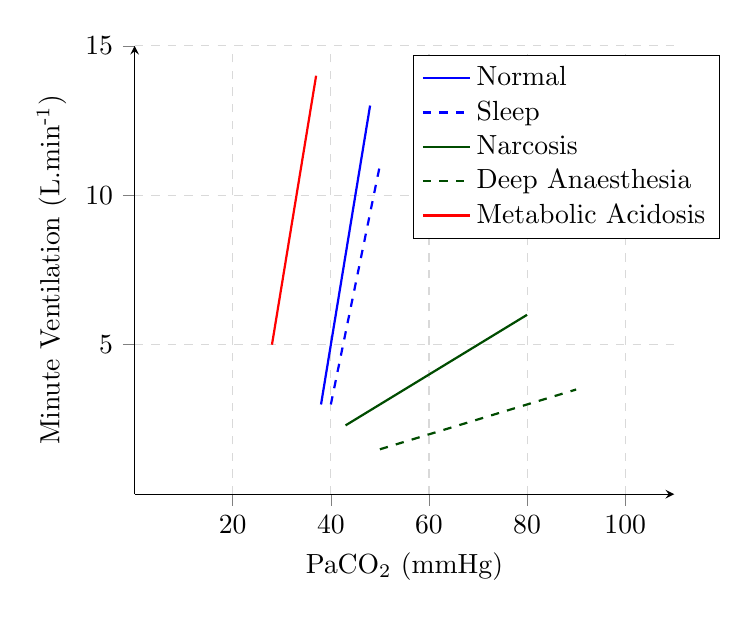
\begin{tikzpicture}
    \begin{axis}[
        axis x line=middle,
        axis y line=middle,
        grid = major,
        grid style={dashed, gray!30},
    	  x label style={at={(axis description cs:0.5,-0.1)},anchor=north},
	  y label style={at={(axis description cs:-0.1,.5)},rotate=90,anchor=south},
        xmin=0,
        xmax= 110,
        ymin= 0,
        ymax= 15,
	 ylabel near ticks,
	xlabel near ticks,
        xlabel=PaCO\textsubscript{2} (mmHg),
        ylabel=Minute Ventilation (L.min\textsuperscript{-1}),
        tick align=outside,
        enlargelimits=false,
legend style={at={(0.8,0.98)},anchor=north},
legend cell align={left}]
	\coordinate (o) (0,0);

	\addplot[domain=38:48, blue, thick,samples=500] {(x-40)+5};
\addlegendentry{Normal}
	\addplot[domain=40:50, blue, dashed, thick,samples=500] {(0.8*x-35)+6};
\addlegendentry{Sleep}
	\addplot[domain=43:80, black!70!green, thick,samples=500] {(0.1*x-5)+3};
\addlegendentry{Narcosis};
	\addplot[domain=50:90, black!70!green, dashed, thick,samples=500] {(0.05*x)-1};
\addlegendentry{Deep Anaesthesia};
	\addplot[domain=28:37, red, thick,samples=500] {x-23};
\addlegendentry{Metabolic Acidosis};

\end{axis}

\end{tikzpicture} 
\end{document}